\documentclass[12pt]{report}
\setcounter{tocdepth}{4}
\setcounter{secnumdepth}{4}
\usepackage{graphicx}
\usepackage{float}
\graphicspath{ {images/} }
\usepackage[
backend=biber,
style=numeric,
citestyle=numeric,
sorting=none]						
{biblatex}							
\addbibresource{mybib.bib}
\setlength{\parskip}{5mm}
\setlength\parindent{0pt}
\usepackage{mathtools}
\usepackage{amsfonts, amsmath, amsthm, amssymb}

\newtheorem{thm}{Theorem}[section]
\newtheorem{lemma}[thm]{Lemma}

\theoremstyle{definition}
\newtheorem{defin}[thm]{Definition}

\theoremstyle{remark}
\newtheorem{rem}[thm]{Remark}
\newtheorem{ex}[thm]{Example}

\usepackage{inputenc}
\usepackage{tikz}
\usetikzlibrary{tikzmark}
\usetikzlibrary{shapes.geometric, arrows}

\tikzstyle{startstop} = [rectangle, rounded corners, minimum width=3cm, minimum height=1cm,text centered, draw=black, fill=red!30]
\tikzstyle{io} = [trapezium, trapezium left angle=70, trapezium right angle=110, minimum width=3cm, minimum height=1cm, text centered, draw=black, fill=blue!30]
\tikzstyle{process} = [rectangle, minimum width=3cm, minimum height=1cm, text centered, draw=black, fill=orange!30]
\tikzstyle{decision} = [diamond, minimum width=3cm, minimum height=1cm, text centered, draw=black, fill=green!30]
\tikzstyle{arrow} = [thick,->,>=stealth]
%Are there any preferred bibliography style choices / general style requirements when it comes to the Maturaarbeit at the KSZ which I ought to implement?

% There are more or less none. Personally I like the notation where you use the
% first letter of the authors surname in square brackets. I think this is also
% the latex preset.  You are free to chose the notation you like most but use it
% consistently. Make sure you include all the information needed in the
% bibliography. If you cite web resources, make sure you include the date you
% retrieved the information. Try to avoid citing Wikipedia but use Wikipedia to
% find other, more credible sources.


\begin{document}

\title{OTP and AES: A historical transition between two systems of cryptography}
\author{Valdemar Thanner\\Supervised by Mr. Bernhard Keller\\Linguistic supervision by Ms. Margrit Oetiker}
\date{23.01.2017}
\maketitle

\chapter*{Dedication}

\chapter*{Acknowledgements}

\chapter*{Introduction}
With the advent of the internet, cryptography has, for the first time in human history, become an integral part of human life. It protects our private communications, safeguards our finances and so much more. In writing this paper, it is my aim to shed some light on the modern cryptography which has become so integral to our daily lives.

However, in order to understand modern cryptography, the foundation upon which it was built, as well as the transition between the two, must also be understood. This is why I have chosen to write about two systems of cryptography: AES, the current standard of cryptography, as well as OTP, which was the first cryptographic algorithm which to be implemented with the help of a computer.

In order to facilitate the examination of how modern cryptography, which was built on the foundation of OTP, affects our lives today, the algorithms AES and OTP must first be fully understood. This is the purpose of the first two chapters; the final chapter will be examining the historical relation between these two incredibly significant algorithms, as well as why cryptography is more important to the everyday person than ever before, and how this came to be.

\tableofcontents

\chapter{OTP: The One Time Pad}

\section{What is a "One Time Pad"?}
When speaking about OTP, it is important to distinguish between its two meanings: On the one hand, it is a technique used to encrypt information. This technique requires one single key, used both to encrypt and decrypt the information. This key is also referred to as a one time pad; therefore, it is important to distinguish between the one time pad (a cryptographical technique) and a one time pad (a key which is used to encrypt and decrypt information).

The One Time Pad is largely derived from the Vernam cipher, which is named after Gilbert Vernam. The Vernam cipher utilized a perforated tape (one of the earliest types of data storage) as the secret key\cite{VernamPatent}. Each bit of data was stored in the form of a hole punched into the perforated tape.

\begin{figure}[H]
\centering
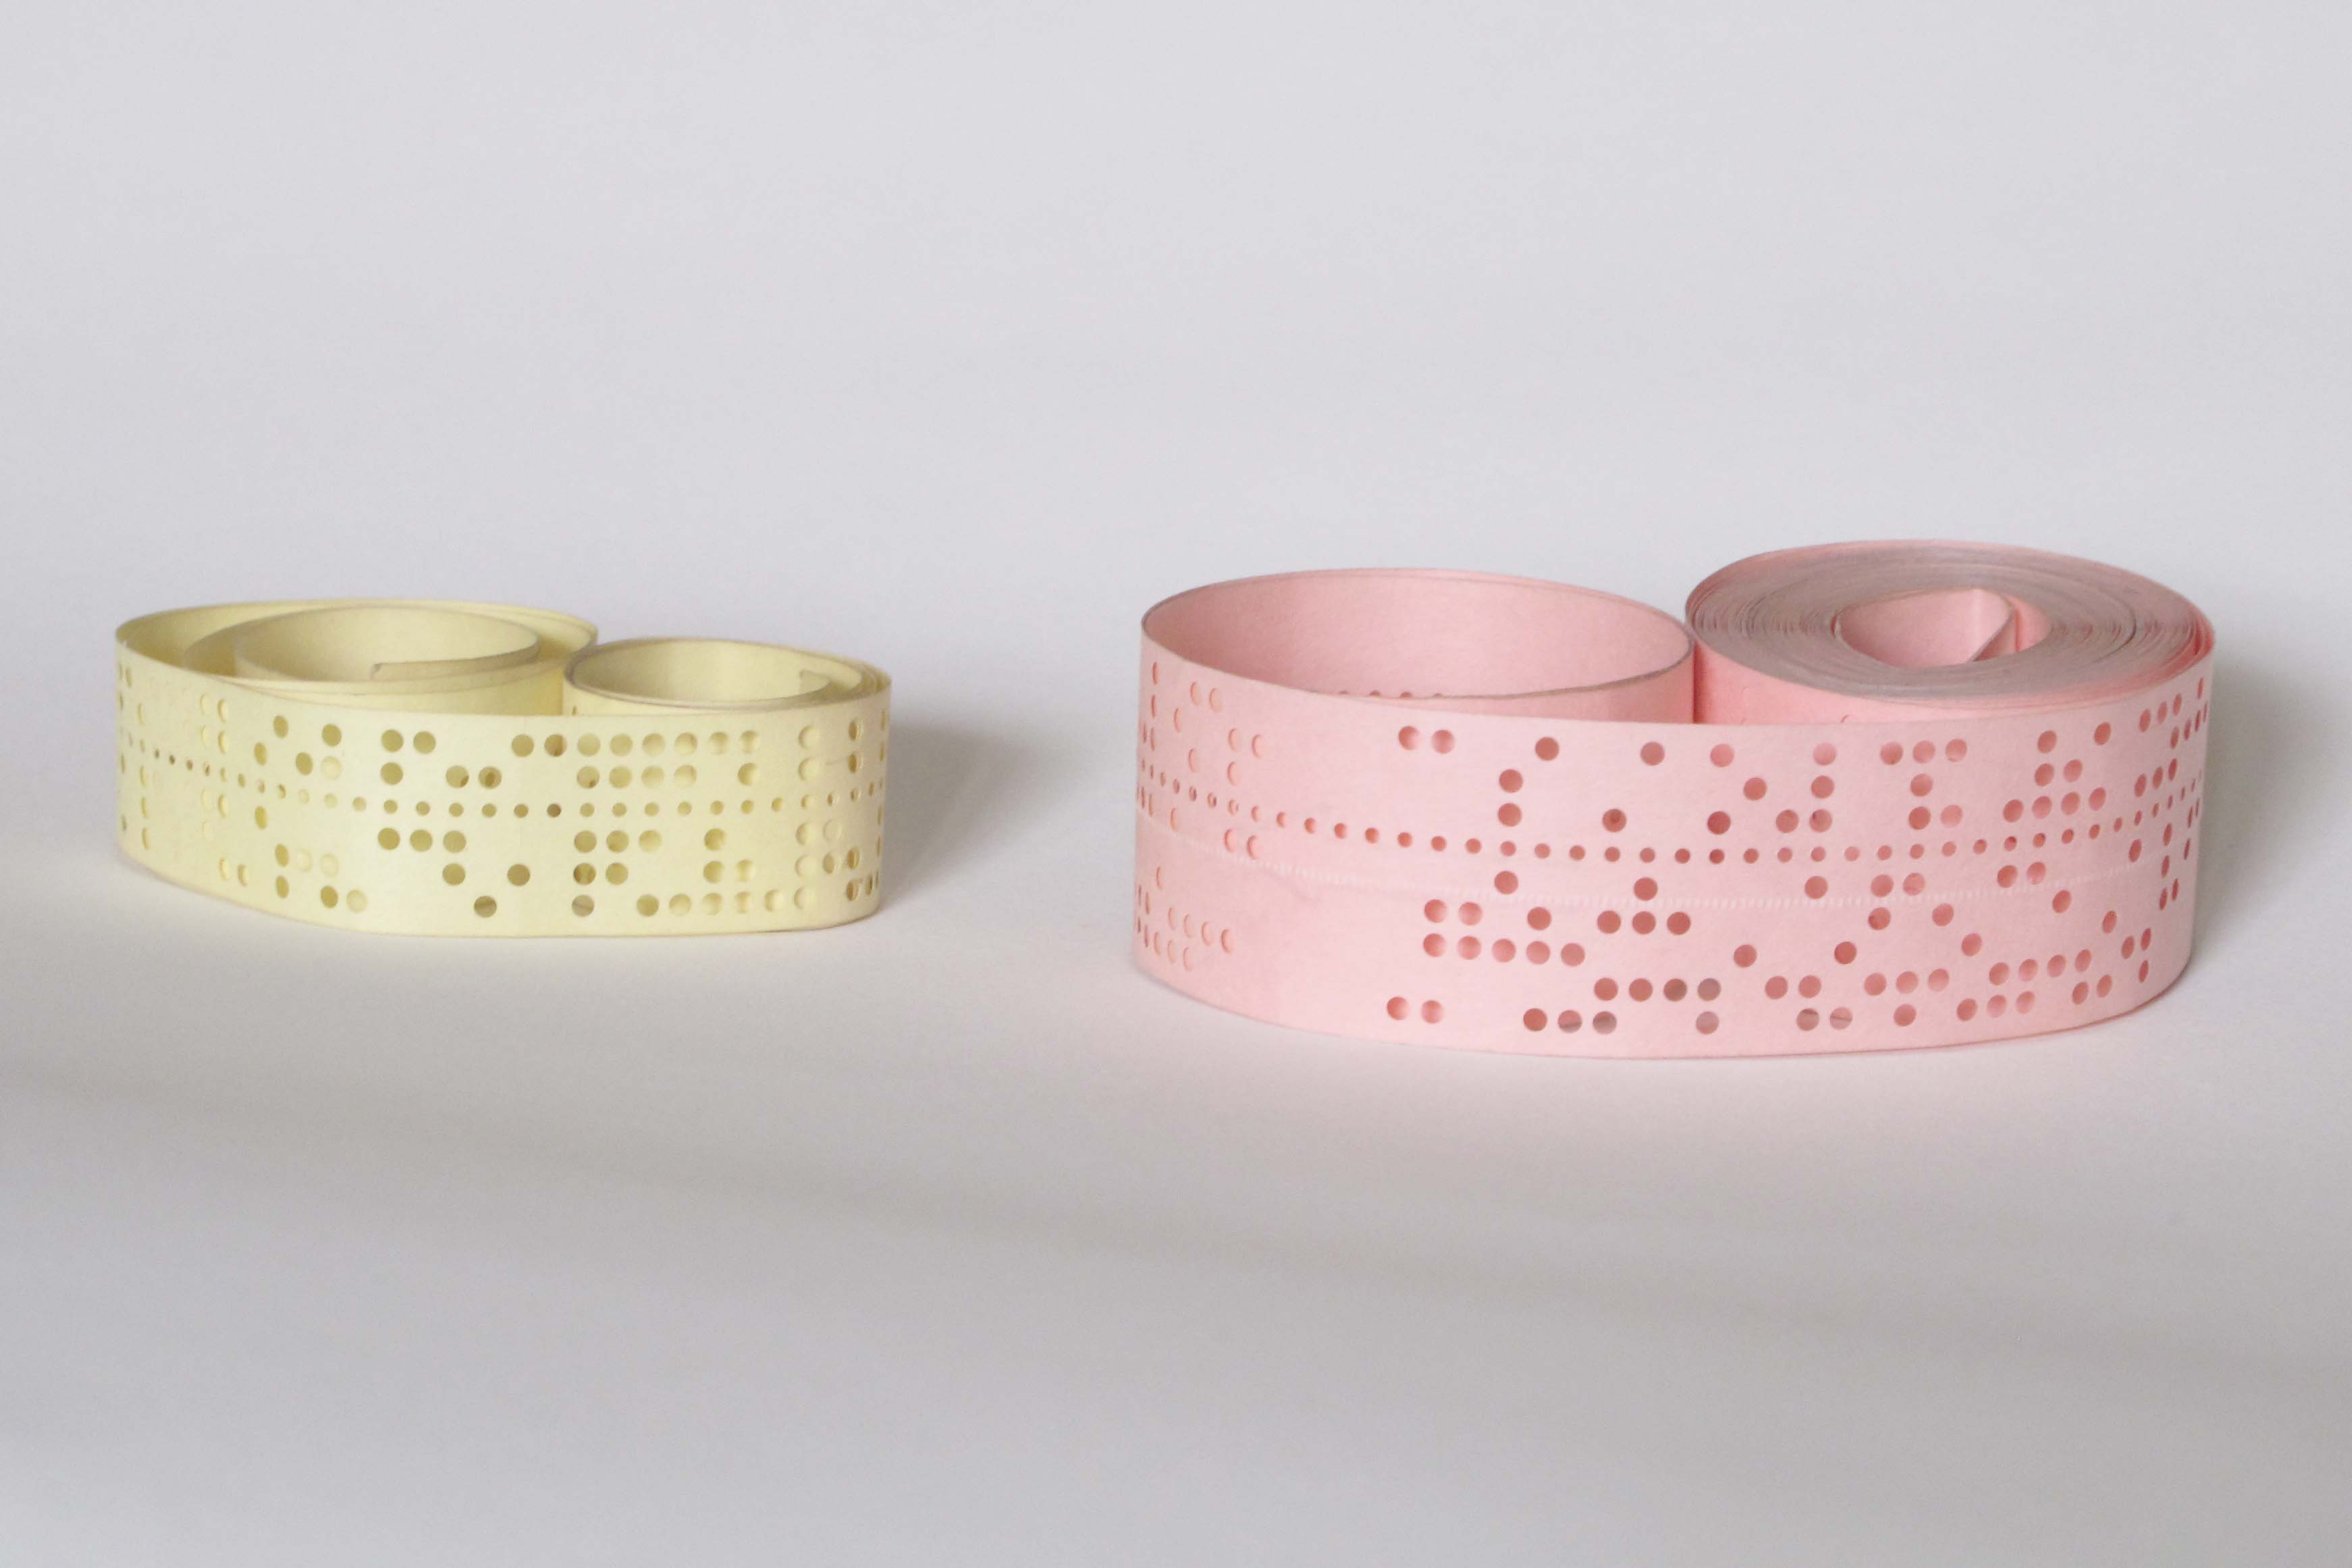
\includegraphics[scale=0.5]{PerforatedTape}
\caption{Perforated tape, utilized to store bits as punched holes}
\end{figure}

However, this system had a vulnerability which the One-Time Pad solved: In Vernam's original method, the perforated tape was not exchanged after it had completed one cycle; instead, it was looped around continuously, often being used to encrypt multiple different messages.

This made the entire system vulnerable. The re-usage of the key meant that the resulting ciphertext suffered from a so-called known-plaintext vulnerability \cite{HutSix}. This means that, if a plaintext and its corresponding ciphertext are captured, the key utilized to generate the ciphertext can be derived from them. This is not an issue if the key is exchanged each time a new message is encrypted. However, if the key of any Vernam cipher machine was compromised through a known-plaintext attack, any further intercepted ciphertexts could be decrypted.

\begin{figure}[H]
\centering
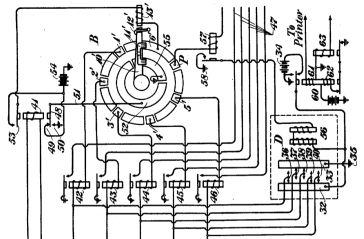
\includegraphics[scale=1]{VernamCipher.jpg}
\caption{A technical diagram from Vernam's famous "Secret signaling system" patent of 1919.}
\end{figure}    

\section{Method used}
%This section, especially the practical example, is the most important part of the chapter.
In the following section, the utilized method will be clarified through usage of an example. In this example, the message \textit{"cryptography"} will first be encrypted by its sender, sent to its intended recipient, and finally decoded by the recipient.

\subsection{Generation of the random key}
In order to encrypt the plaintext, a key must first be generated. This key will be utilized to encrypt the plaintext through the usage of modular addition, turning it into the ciphertext.

This key must fulfil some crucial criteria \cite{MilsElectronic}. Foremost, the length of the key (the amount of  characters contained within it) must be equivalent to or greater than the length of the plaintext; otherwise, it is not possible to perform any encryption (using the OTP). Secondly, the key must be generated randomly. This is mainly due to the fact that a randomly generated key makes frequency analysis\cite{FrequencyAnalysis}, the form of cryptanalysis most commonly used to break classical ciphers, impossible.

% It's not clear what it means to generate a key randomly. 

The key consists of numbers. Usually, when the plaintext is made up of Latin letters, the numbers range between 0 and 25. The key can be converted into Latin letters through the same method applied to the plaintext outlined in the following chapter, however, this is not necessary, although the key is often transported in the form of text.

As the message being encrypted in this example has 12 characters, the key must also posses at least 12 characters. For the sake of this example, the key \textit{"sytruifgnihm"} will be utilized.

\subsection{Modular addition of the key and plaintext}
%unsure if a picture explaining modular addition and subtraction is needed, or if the provided explanation suffices?			

% In my opinition, the part about modular addition is quite clear. You could
% also add a binary example where you don't even need the concept of modular
% addition since all you need is an XOR gate - which of course is the same as
% modular addition of bits - but easier to understand.


Next, the ciphertext is created through modular addition of the key and the plaintext. This can be applied not only to a message consisting of alphabetical characters, but also to any sequence of bits. If the plaintext consists of a message made up of alphabetical characters, the plaintext and the key are added using arithmetic referred to as \textit{"addition modulo 26"}. The correct mathematical notation for modular arithmetic is $(a+b)\:mod\:c$, where c is referred to as the \textit{modulus}, which is the value that cannot be passed nor reached in modular addition. In order to perform modular addition, the variables a and b are first added, after which they are divided by the modulus c, up to an integer. The resulting remainder r is the final result of the operation.

Before the modular addition of the plaintext and the key can begin, each character (of the plaintext as well as of the secret key, in the case that the key was generated as a string of Latin letters instead of as a sequence of numbers) must be converted to a number, corresponding to it's position in the Latin alphabet:

\begin{figure}[H]
\centering
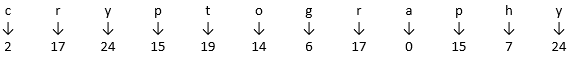
\includegraphics[scale=1]{Table1.PNG}		
\end{figure}
%Do these tables suffice in aiding understanding the example, or 		                                             should I include more "graphical" explanations as well?

% I don't think this needs to get any more graphical. You could look into latex
% tables and math syntax for arrow to make the typesetting look a bit more
% consistent.

As the key was also generated in the form of characters, it too must be converted to a sequence of numbers:

\begin{figure}[H]
\centering
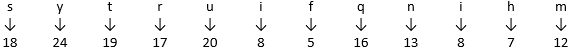
\includegraphics[scale=1]{Table2.PNG}
\end{figure}

Afterwards, the key and the plaintext are added together utilizing modular addition. Of course, all operations below are performed in \textit{mod 26}. Finally, the resulting numbers are converted to the character to which they correspond in the Latin alphabet. The resulting sequence of characters is referred to as the ciphertext.

\begin{figure}[H]
\centering
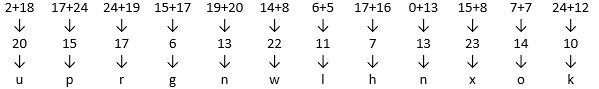
\includegraphics[scale=1]{Table3.PNG}
\end{figure}

The modular addition of the plaintext and the key can also, however, be performed bitwise. This simply means that, instead of adding a message consisting of (up to) 26 different letters with a key (also consisting of up to 26 different letters), we simply add the bits of the plaintext (a computer file consisting of bits), which can assume the value of either 1 or 2, with the bits of the key. The bits are added in modulo 2. This process is referred to as XOR, one of the basic bitwise operations which can be performed directly by a computers central processor.

\begin{figure}[H]
\centering
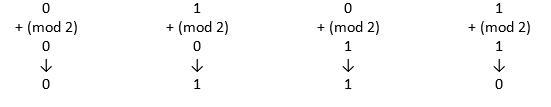
\includegraphics[scale=1]{XORgate.PNG}
\caption{The formula used by an XOR gate.}
\end{figure}

\subsection{Decoding of the ciphertext using the key}
Assuming the message has been delivered to the intended recipient, who must hold a copy of the secret key (which, as OTP is a symmetrical cryptographical method, is identical to the one utilized to create the ciphertext), the recipient can now decode the ciphertext in order to view the plaintext.

Since the ciphertext was created through the modular addition of the plaintext and the key, the recipient can utilize modular subtraction in order to view the plaintext. In order to do this, the recipient must subtract the key from the ciphertext in modulo 26, and convert the resulting numbers to Latin characters.  However, it is now also necessary for the numbers not to become negative. Fortunately, this is also made possible by modular arithmetic, as the values simply loop back around from 0 as well. Once again, all below operations are in \textit{mod 26}.

\begin{figure}[H]
\centering
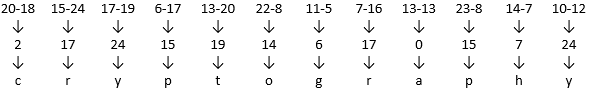
\includegraphics[scale=1]{Table4.PNG}
\end{figure}

Now, the message's journey is complete, having passed from plaintext into ciphertext, being transported to its intended recipient in the form of ciphertext, and finally being decoded and read by its recipient. 

\section{Perfect secrecy: Information-theoretical security}
An important characteristic of perfect secrecy is that the ciphertext conveys no information at all in regards to the plaintext; this means that it is not possible to garner any information about the key nor the plaintext if one is in possession of the ciphertext \cite{PerfectSecrecy} \cite{HandbookOfAppliedCryptography}. In probability theory, where $C$ contains all possible ciphertexts and $M$ contains all possible messages:

\begin{defin}\label{def:perfectsecrecy}
$for c \in C: \\
\forall m_1, m_2 \in M: \\
P(E_k(m_1)=c) = P(E_k(m_2)=c)$
\end{defin}

$E_k$ is a defined as a cipher using the key $k$ if there exists a function $D_k(m)=c$, also using the key $k$, which decrypts each ciphertext to a unique message.

From this, two other important characteristics of a cryptographical system with perfect secrecy can be derived. Firstly, perfect message indistinguishability. This means that, even if you are provided with multiple different plaintexts and one ciphertext, it is impossible to assign any one plaintext to the provided ciphertext. Secondly, if the key is the same length as the plaintext (as is the case in OTP), then there exists a key for every possible encryption from plaintext to ciphertext. This means that any plaintext can be converted to any ciphertext, making it impossible to determine the key without access to both the plaintext and the ciphertext. This is referred to as perfect key ambiguity.		%This paragraph was difficult for me to summarize well.

Although many believe that the ciphertext does provide information about the plaintext, namely its length, this can easily be solved through padding, where characters of no importance to the plaintext are added to it before encryption \cite{HutSix}.

\subsection{Mathematical proof}
%This is the section which was most difficult for me to write; I opted to present a more simplified explanation of %Shannons proof without the use of probability theory.
%Should I Include the probability Theory or is it better to keep it simple for the reader?

% I'm not convinced that you'll manage to present a mathematically correct proof without using
% any probability theory. There are a few problems with the current version of the proof: 


%In 1949, Shannon proved the perfect secrecy of OTP by using probability theory \cite{ShannonOTP}. To be precise, he proved that, in order to achieve perfect secrecy, the key must possess at least the same length as the plaintext; one of the key characteristics of OTP. If this is the case, then an attacker cannot determine the plaintext given the ciphertext, even with access to infinite computational capacity; a "brute-force attack" is impossible.

% To proof that OTP provides perfect secrecy it's not enough to show that one
% can only achieve perfect secrecy with a key of the same length as the message
% as this is only a necessity but no sufficiency
% (https://en.wikipedia.org/wiki/Necessity_and_sufficiency) to achieve perfect
% secrecy. E.g. if I use the key consisting of as many zeros as the message has
% letters and encrypt every message by adding said key, the encryption gives you
% no secrecy at all even though the key has the same length as the message.


%A simplified method of presenting this proof is as follows:
%
%If the attacker does indeed possess infinite computational capacity, he can generate every possible key which could have been used to generate the ciphertext, and he can then generate every possible plaintext (each of which will correspond to the given ciphertext and one of the generated keys).

% I don't understand the comment in brackets. You could use a graphical explanation or mathematical
% notation to make your point clearer.

%It follows that, if the ciphertext was $m$ bits long, there would be $2^m$ possible keys (or, in the case that the plaintext and ciphertext consist of Latin characters, $26^m$ possible keys). This is because a bit can possess the value of either 0 or 1, meaning that each individual bit of the key has two possible values. As The entire key possesses m bits, each cell must be multiplied by the following cell in order to obtain the total number of possible keys. In the case that the key consists of Latin characters, however, each cell possess 26 possible values (ranging from 0 to 25); therefore, the total number of possible keys would be $26^m$.

%If the possible amount of keys that the attacker can generate is equal to $2^m$, and the attacker can generate one possible plaintext for each key, that means that the amount of plaintexts which the attacker can generate is also equal to $2^m$ (or, once again, in the case of Latin characters, equal to $26^m$ plaintexts).
%
%This amount, $2^m$, is equal to the amount of possible bit sequences of the length m; therefore, the attacker cannot possibly eliminate any one possible plaintext of the length m, meaning that he cannot garner any information from the ciphertext on its own. This fulfils the requirements of perfect secrecy.

% We should discuss the above paragraphs in a meeting as I don't fully
% understand what you are trying to say. I'm not convinced that this suffices to
% proof perfect secrecy. Most importantly, it appears that you never used the
% randomness of the key in your proof. That's also the point where it gets
% difficult to avoid probability theory. Without probability theory you don't
% have a understanding of what it means for a key to be ``random''.

In 1949, Shannon proved that OTP did, in fact, posess perfect secrecy\cite{ShannonOTP}. First, the properties and contents of the sets and variables used in this proof must be clarified:

\begin{defin}
Let $M$ contain all possible messages; meaning all possible bit sequences.

Let $m$ be the plaintext. $m \in M$.

Let $c$ be the ciphertext.

Let $K$ contain all possible keys.

Let $k$ be the key. $k \in K$.

Let the function ${E_k}(m)=c$. The function $E$ is an encryption process using the key k, which outputs the ciphertext $c$ using the plaintext $m$.

Let $m^{*}$ be a possible message, selected at random using a uniform distribution:
$\forall m^{*} \in M: P(m^{*})=\frac{1}{\lvert M \rvert}$

Let $k^{*}$ be a possible key, selected at random using a uniform distribution.
$\forall k^{*} \in M: P(k^{*})=\frac{1}{\lvert K \rvert}$
\end{defin}

\begin{lemma}
In order for perfect secrecy to apply, then:

$P( m=m^{*} \mid E(m)=c ) = P( m=m^{*} )$
must be true, fulfilling the definition of perfect secrecy \ref{def:perfectsecrecy}

\begin{rem}
This is because, if the probability that the actual plaintext $m$ is equal to some other message $m^{*}$, given the ciphertext $c$, is equal to the probability that $m=m^{*}$, then the ciphertext $c$ provides no additional information to the attacker. The ciphertext not providing any information about the plaintext nor the key is the definition of perfect secrecy; therefore, if the above equation can be proven to be true in the case of OTP, then the perfect secrecy of OTP will also have been proven.
\end{rem}
\end{lemma}

\begin{thm}
$P( m=m^{*} \mid E(m)=c ) = P( m=m^{*} )$ is true in the case of OTP.
\end{thm}

\begin{proof}
Per the definition of conditional probability, 

$P(m=m^{*} \mid {E_k}(m)=c) = \frac{P(m=m^{*} \cap {E_k}(m)=c)}{P({E_k}(m)=c)}$.

First, the computation of $P({E_k}(m)=c)$:

\begin{rem}
The distribution of the messages is not uniform, as it must be assumed that a potential attacker has some form of knowledge about the nature of the message. Therefore, each message is not equally likely, meaning that 
$P(m=m^{*}) \neq \frac{1}{\lvert M \rvert}$. $P({E_k}(m)=c)$ can also be taken as $P(k=k^{*})$, because the probability of the function encrypting a certain message into a certain ciphertext hinges solely on the key. As the key is randomly generated, each possible key is equally likely. Therefore, 
$P(k=k^{*}) = P({E_k}(m)=c) =  \frac{1}{\lvert K \rvert} $.
The mathematical computation of $P({E_k}(m)=c)$ reaffirms this conclusion.
\end{rem}

In order to find the probability that the given key $k$ maps the given message $m$ to the given ciphertext $c$, all probabilities that a certain key-message pair, $k_i$ and $m_i$, encrypt to the given ciphertext $c$, are summed up. This summation needs to be divided by the probability space. Because each key is applied to each message, the probability space is $\lvert M \rvert*\lvert K \rvert$.

\begin{tabular}{cccc}
$k_0$\tikzmark{a} & \tikzmark{z}$k_1$\tikzmark{b} & ... & $k_{\lvert K \rvert}$\tikzmark{c} \\
 & & & \\
$m_0$\tikzmark{d} & \tikzmark{e}$m_1$\tikzmark{y} & ... & \tikzmark{f}$m_{\lvert M \rvert}$ \\
\end{tabular}


\begin{tikzpicture}[overlay, remember picture, yshift=.25\baselineskip, shorten >=.5pt, shorten <=.5pt]
\draw [->] ({pic cs:a}) [bend left] to ({pic cs:d});
\draw [->] ([yshift=.75pt]{pic cs:a}) -- ({pic cs:e});
\draw [->] ([yshift=.75pt]{pic cs:a}) -- ({pic cs:f});
%\draw [->] ({pic cs:b}) [bend left] to ({pic cs:y});
%\draw [->] ([yshift=.75pt]{pic cs:z}) -- ({pic cs:d});
\end{tikzpicture}

$P({E_k}(m)=c) = \sum\limits_{\substack{m_i \in M \\ k_i \in K}}
P(E_{k_i}(m_i)=c) 
* \frac{1}{\lvert M \rvert*\lvert K \rvert}$

In OTP, there exists exactly one key which maps a specific message to a specific ciphertext. Therefore:

$\sum\limits_{k_i \in K}
P(E_{k_i}(m_i)=c)
=1$

$\sum\limits_{m_i \in M} 1
= \lvert M \rvert$

$\Rightarrow P({E_k}(m)=c) = \frac{\lvert M \rvert}{\lvert M \rvert*\lvert K \rvert} = \frac{1}{\lvert K \rvert}$

\begin{rem}
Note that, due to the above mentioned possibility that the attacker possesses some knowledge of the message, $P(m=m^{*}) \neq \frac{1}{\lvert M \rvert}$. Therefore, $P(m=m^{*})$ cannot be further simplified. In order to find $P(m=m^{*} \cap {E_k}(m)=c)$, the definition of conditional probability as well as the property $P({E_k}(m)=c) = \frac{1}{\lvert K \rvert}$ are used.
\end{rem}

$P(m=m^{*} \cap {E_k}(m)=c) = \frac{P(m=m^{*})}{\lvert K \rvert}$

Now, the values computed for $P({E_k}(m)=c)$ and $P(m=m^{*} \cap {E_k}(m)=c)$ are inserted into the left hand side of the equation to see if it equals the right hand side of the equation.

$\dfrac{\dfrac{P(m=m^{*})}{\lvert K \rvert}}{\frac{1}{\lvert K \rvert}} = P(m=m^{*}) \\
= RHS$
\end{proof}

\subsection{Consequences of the proof}
%Not sure if this information warrants its own section or if I should merge it with the above one

%From the above proof, it can be concluded that, in order for the elimination of any possible %plaintext to be impossible (rendering a brute-force attack impossible), the key must possess %at least the same length as the plaintext. Also, the individual bits of the must not be %dependant on one another. These conditions are only fulfilled by OTP.

The most important conclusion which Shannon drew from his proof was that, in order for a cipher to posess perfect secrecy, $\lvert K \rvert \geqslant \lvert M \rvert$\cite{ShannonOTP}. This means that the key needs to be at least as long as the message. Note that using a key as long or longer than the message does not, however, constitute guaranteed perfect secrecy: It is merely an absolute necessity.

\section{Issues with OTP}
%I had just one sentence here, but felt it appeared strange to just have one sentence and opted to leave it blank.
\subsection{True randomness in generating the key}
One of the most important aspects of the utilized key is that it must be completely random (see 1.2.1). However, generating a random sequence of numbers or letters is no trivial task. In fact, most random number generation functions of even modern programming languages are not adequately random for use in cryptography. This is especially difficult for computers, considering that a computer is, in essence, designed to follow a set of predictable instructions as quickly as possible.

Therefore, in order to generate a sufficiently random key, it is preferable to utilize hardware random number generators, for example by utilizing a true random noise source \cite{MilsElectronic}. One such example is the key generator built by mils electronic, where a set of parallel ring oscillators are sampled. Because the oscillation speed of each ring is influenced by random factors such as local variations in temperature and voltage.

\begin{figure}[H]
\centering
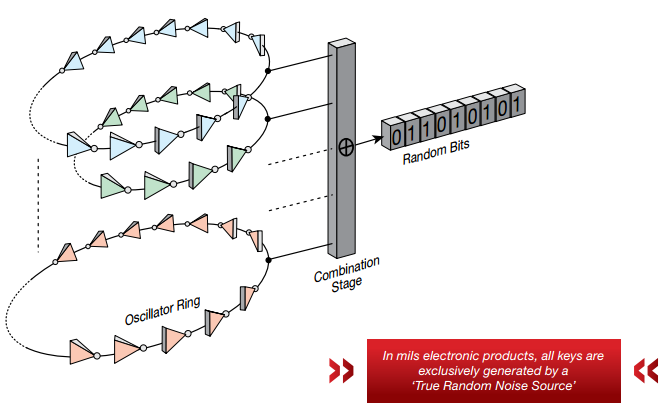
\includegraphics[scale=0.75]{MilsElectronic.PNG}
\caption{A hardware random number generator with sufficient randomness to be utilized in the generation of one-time pads.}
\end{figure}

\subsection{Secure distribution of the key itself}
The main issue in regards to OTP is that, while it posses perfect security, therefore solving the issue of safely transmitting the ciphertext, the problem instead becomes how to securely transmit the key to the intended recipient of the encrypted message.

Therefore, in order to ensure that the plaintext cannot be accessed by any party other than its intended recipient, the complete security of the transmittal of the key must also be ensured.

However, if the communicants already possess a method by which the key can be transmitted with infallible security, then it stands to reason that the plaintext itself could just as well be submitted through the same channel, considering that it has the same number of bytes (or characters) as the key. So, the problem of securely transmitting the plaintext has simply been transferred to the problem of securely transmitting the key.

One method of mitigating this issue is to first send one very long key, which can then be used for multiple messages in the future. Using this method, only one secure transmission has to be made in order to ensure the security of multiple transmissions. 

\subsection{Secure disposal of a utilized key}
%Once again, not entirely sure if this warrants its own section or if it should be merged into the above section.
After a key has been fully utilized, it has to be disposed of securely, in order to prevent any information from being compromised in the future, which is possible should the key continue to exist. Therefore, it is necessary to completely eradicate the entirety of the key. If the key was stored on a digital media, such as a USB drive or HDD, the only completely secure method of disposal is considered to be complete incineration.

% Whenever you use a sentence like ``is considered to be...'' you need to
% provide a source. Are you sure that incinerating hard drives does the job? The
% ways I know of used to destroy harddrives involve strong electromagnets and drills.

\chapter{AES: The Advanced Encryption Standard}

\section{AES viewed from a high level}

Viewed from a high level, the AES algorithm consists of one XOR step, followed by 10 rounds of cryptographical measures, with each round as well as the initial XOR step using a specific subkey, generated using the main key. By passing through these steps, each block of plaintext is converted into a block of Ciphertext. In the following chapter, each individual aspect of the complete AES algorithm will be more closely examined.

\begin{figure}[H]
\centering
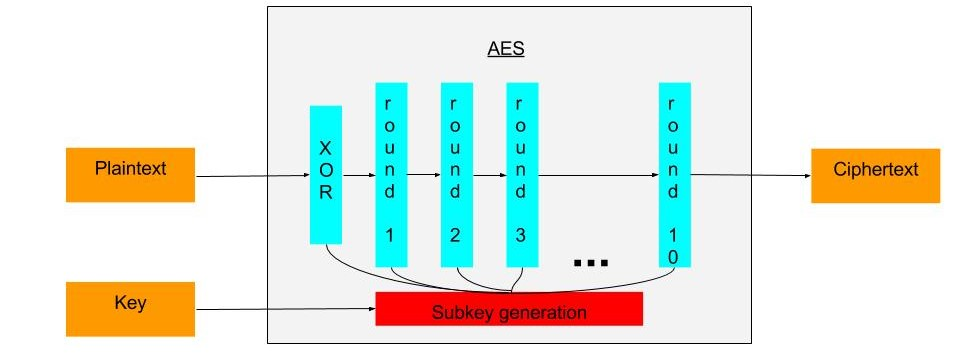
\includegraphics[scale=0.4]{AES_fig1.jpg}
\caption{A high-level description of AES.}
\end{figure}

\section{Encryption}
Each round possesses 4 steps, explained in detail below. However, before those operations can be understood, some basic terminology must first be clarified.

The "state" is the matrix containing the information which is manipulated throughout the encryption process. As such, the state begins its journey through AES as the block of plaintext which is to be encrypted, and ends it as a block of ciphertext. The state is represented in a $4 \times 4$ column-major order matrix, meaning that the bytes are counted from top to bottom. In a block containing 16 bytes, the standard size of an AES plaintext block as well as the standard size of  an AES key is $(16 bytes \cdot 8 = 128 bits)$.

\[ \left( \begin{array}{cccc}
a_0 & a_4 & a_8 & a_{12} \\
a_1 & a_5 & a_9 & a_{13} \\
a_2 & a_6 & a_{10} & a_{14} \\
a_3 & a_7 & a_{11} & a_{15}\end{array} \right)\] 

However, in order to clarify the manipulations performed throughout the 10 rounds of AES, it is more beneficial to note the starting position each byte takes in the subscript instead of noting its chronological order in the plaintext block.

\[ \left( \begin{array}{cccc}
a_{0,0} & a_{0,1} & a_{0,2} & a_{0,3} \\
a_{1,0} & a_{1,1} & a_{1,2} & a_{1,3} \\
a_{2,0} & a_{2,1} & a_{2,2} & a_{2,3} \\
a_{3,0} & a_{3,1} & a_{3,2} & a_{3,3}\end{array} \right)\] 

Each AES round key possesses the same size as the state, and is made into a matrix in the exact same fashion; this is, of course, necessary for the successful modular addition of the bytes contained within the state and those contained within the subkey using the XOR operation.


\subsection{Initial XOR operation}

\begin{figure}[H]
\centering
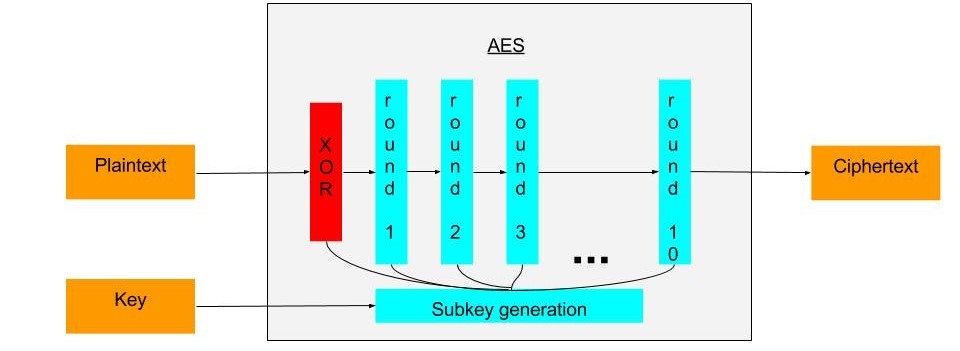
\includegraphics[scale=0.4]{AES_fig2.jpg}
\end{figure}

This step is identical to the XOR operation already described in the chapter regarding OTP. The XOR operation simply represents an addition modulo 2, and is denoted using the symbol $\bigoplus$. Once again, a simple XOR gate is used to add the state with the initial XOR operations own round key, which is identical to the master key (see 2.2.2.3).

\[ 
\left( \begin{array}{cccc}
a_{0,0} & a_{0,1} & a_{0,2} & a_{0,3} \\
a_{1,0} & a_{1,1} & a_{1,2} & a_{1,3} \\
a_{2,0} & a_{2,1} & a_{2,2} & a_{2,3} \\
a_{3,0} & a_{3,1} & a_{3,2} & a_{3,3}\end{array} \right)
\bigoplus
\left( \begin{array}{cccc}
k_{0,0} & k_{0,1} & k_{0,2} & k_{0,3} \\
k_{1,0} & k_{1,1} & k_{1,2} & k_{1,3} \\
k_{2,0} & k_{2,1} & k_{2,2} & k_{2,3} \\
k_{3,0} & k_{3,1} & k_{3,2} & k_{3,3}\end{array} \right)
\]

Here, each byte of the state is combined with the byte of the subkey which possesses the corresponding position using the XOR operation. For example, $a_{2,1}$ would be combined with $k_{2,1}$. The resulting byte is then placed at the matching coordinate (in this example, once again the coordinate 2,1) of the resulting matrix. The completed matrix resulting from this operation is the new state. Next, this resulting state proceeds into the first of ten so-called "rounds".

\subsection{Rounds}

\begin{figure}[H]
\centering
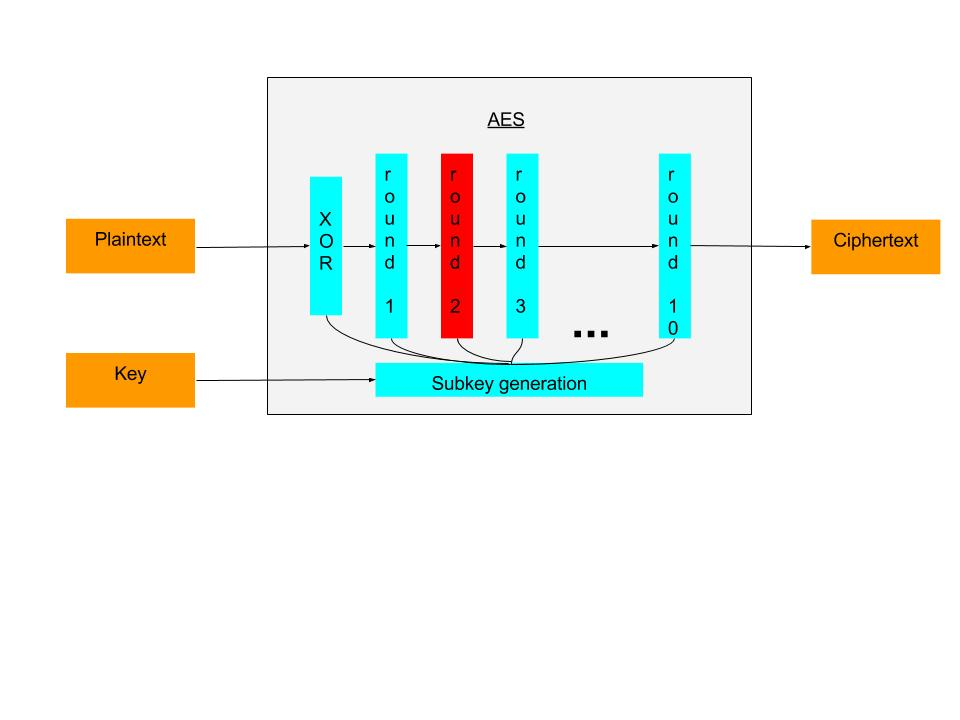
\includegraphics[scale=0.4]{AES_fig3.jpg}
\end{figure}

\subsubsection{Galois Field $GF(2^8)$ arithmetic}
Before the math behind AES can be fully understood, the Galois Field $GF(2^8)$ must first be more closely examined. This field contains only 256 values, ranging from 0-255; the range which can be stored in a byte. Secondly, all bytes are written using hexadecimal notation. Most importantly, all binary strings are represented as polynomials; this is best illustrated through an example \cite{GFieldExample}.

$11001000 = 1x^7+1x^6+0x^4+1x^3+0x^2+0x^1+0x^0 = x^7+x^6+x^3 $ 

$10000111 = x^7+x^2+x+1$

Addition is made rather simple through this; keeping in mind that, since addition is an XOR operation, two identical factors neutralize each other $(x^n+x^n = 0)$.

Therefore, a byte can be written as a polynomial, in binary or in hexadecimal\cite{BinHex}.

$(x^7+x^6+x^3)+(x^7+x^2+x+1) = x^6+x^3+x^2+x+1 = 01001111 = 4f$

As can be seen, this method is in keeping with the XOR addition of bytes. However, multiplication within the field is not quite as simple.

The issue with multiplying two bytes with each other within the finite field is that it is possible to receive a polynomial of higher order than 7; polynomials like this cannot be stored as a byte. Therefore, a reducing polynomial of the order 8 must be utilized. AES defines this reducing polynomial as $x^8+x^4+x^3+x+1$. The Galois Field $GF(2^8)$ utilizing the reducing polynomial $x^8+x^4+x^3+x+1$ for multiplication is referred to as Rijndael's finite field\cite{RFiniteField}.

In order to prevent a result that cannot be stored as a byte, all results of multiplications between bytes are then taken modulo the reducing polynomial. This means that, if the degree of a resulting polynomial exceeds 7, an XOR division using the reducing polynomial must be performed.

\subsubsection{Finding the multiplicative inverse using the extended euclidean algorithm}
The multiplicative inverse of a number is defined as equalling one when multiplied with the number in question. The multiplicative inverse of $a$ is $a^{-1}$, as $a^{-1} \cdot a = 1$. Taking a variable to the power of $-1$ is defined as finding the multiplicative inverse.

In AES, it is often necessary to find the multiplicative inverse of a byte. Furthermore, this multiplicative inverse must be found within the Rijndael field, meaning the multiplicative inverse must be found modulo the reducing polynomial. To this end, the extended euclidean algorithm is used.

The regular Euclidean algorithm is simply a computationally efficient method to find the greatest common divisor of two positive integers. In order to find the gcd, the Euclidean algorithm checks how many times the smaller integer goes into the larger one, leaving r over. The algorithm then checks how many times r goes into the smaller integer, continuing in this manner until $r=0$. Once this point has been reached, the last value before r=0 is the gcd.

$a = k \cdot b + r$

Next, assign b to a and r to b: $a=b, b=r$
 
Continue to repeat these steps until $r=0$.

The regular euclidean algorithm can be applied to polynomials over a finite field, such as Rijndael's finite field, with no issues as long as the rules of the field are observed\cite{EuclideanPolynomials}.

The extended Euclidean algorithm is used to compute the integers $x$ and $y$ $({x,y} \in \mathbb{Z})$ of B\'ezouts Identity\cite{Bezout}, in order to fulfil the following equation:

$ax+by = gcd(a,b)$

The following example uses $a=240$ and $b=46$.

\begin{center}
$\begin{vmatrix}
r_k & x_k & y_k & q_k \\
240 & 1 & 0 & 1 \\
46 & 0 & 1 & 5 \\
10 & 1 & -5 & 4 \\
6 & -4 & 21 & 1 \\
4 & 5 & -26 & 1 \\
2 & -9 & 47 & 2 \\
0 &  &  &  \end{vmatrix}$
\end{center}

The starting conditions of the algorithm are always identical: $x_0=1, x_1=0$ and $y_0=0, y_1=1$. Next, the largest value of $a$ and $b$ is placed in $r_0$ (in this case 240), with the smaller value being placed in $r_1$ (in this case 46). The quotient q is how many times 46 goes into 240, namely 5 times. The remainder of 10 is then placed into the next spot in the $r_k$ column. Now, $x$ and $y$ can be computed:
$x_2=x_0-x_1 \cdot q_1 \Rightarrow 1=1-0 \cdot 5$

$y_2=y_0-y_1 \cdot q_1 \Rightarrow -5=0-1 \cdot 5$

This can be used to calculate all $x_k$ and $y_k$ values\cite{EuclidGeneralization}:

$x_k=x_{k-2}-x_{k-1} \cdot q_{k-1}$

$y_k=y_{k-2}-y_{k-1} \cdot q_{k-1}$

All columns are then filled using this method until a value in the $r_k$ column reaches 0. At this point, the values in the row above the 0 are the answers to the equation $ax+by = gcd(a,b)$.

Within Rijndael’s finite field, this becomes more complicated, as the algorithm must be applied within a finite field which employs a reducing polynomial.

Since the reducing polynomial is $x^8+x^4+x^3+x+1$, the equation that must be solved to find the multiplicative inverse of the polynomial $p$ goes as follows:

$a \cdot p+b \cdot (x^8+x^4+x^3+x+1) = 1 = gcd(p, x^8+x^4+x^3+x+1)$

$b \cdot ( x^8+x^4+x^3+x+1) = 0$

$a \cdot p = 1$

$\Rightarrow a = p^{-1}$

All operations within the field are performed modulo the reducing polynomial. Therefore, the gcd of the reducing polynomial and any other polynomial is always equal to one.

In order to find the multiplicative inverse of $p$, namely $a$, the extended euclidean algorithm can be applied. As always, it is of great importance that the rules of the field are observed.

\subsubsection{Round key generation (KEYEXPANSIONS)}
As can be seen in the high-level explanation, AES requires 11 128-bit subkeys (also referred to as round keys); one for the initial XOR operation, and then one for each of the 10 rounds. These subkeys are derived from the master key using the "Rijndael key schedule" \cite{KeySchedule}. In the most basic implementation of AES, the master key has a length of 128 bits. There are also implementations of AES using keys of lengths 192 and 256 bits. Such longer keys are used to provide even greater security, and are considered standard for top-secret documentation\cite{CNSSPolicy}. It is important to note that, even though the key size varies, AES always retains the same block size.

The first round key, utilized for the initial XOR operation, is simply the master key itself.

\[ \left( \begin{array}{cccc}
k_0 & k_4 & k_8 & k_{12} \\
k_1 & k_5 & k_9 & k_{13} \\
k_2 & k_6 & k_{10} & k_{14} \\
k_3 & k_7 & k_{11} & k_{15}\end{array} \right)\] 

Each subsequent round key must be generated through key expansion, using the master key as a template for the generation of the first round key.

The first four bytes of the 16-byte round key, which are contained within the first column of the round key matrix, are generated first. To this end, the last, as in the rightmost, column is stored in a temporary variable, for example x. The so-called RotWord operation is then employed, wherein each byte is transposed one step upwards.

\[
\left( \begin{array}{c}
x_0 \\
x_1 \\
x_2 \\
x_3\end{array} \right)
\xrightarrow{\text{RotWord}}
\left( \begin{array}{c}
x_1 \\
x_2 \\
x_3 \\
x_0\end{array} \right)
\]

Afterwards, the four bytes resulting from the RotWord operation are each replaced through utilization of a Rijndael S-Box (see  2.2.2.2). The resulting vector now needs to be added to the first, as in the leftmost, column of the master key using an XOR gate.

\[
\left( \begin{array}{c}
x_1 \\
x_2 \\
x_3 \\
x_0\end{array} \right)
\xrightarrow{\text{SubBytes}}
\left( \begin{array}{c}
b_0 \\
b_1 \\
b_2 \\
b_3\end{array} \right)
+
\left( \begin{array}{c}
k_0 \\
k_1 \\
k_2 \\
k_3\end{array} \right)
\]

The final step to obtain the first four bytes of the round key is referred to as the RCon, meaning round constant step\cite[p. 15]{Rijndael}. In this step, a vector dependent on the iteration, the chronological number of the round key being generated starting with one, is added using an XOR gate. These vectors are constant for every application of AES; for example, the RCon vector obtained using an iteration of eight will always be used in the process of obtaining the first four bytes of the eighth round key.

The RCon vector is calculated through the following formula, with i standing for the iteration.

\[ \left( \begin{array}{c}
{02}^{i-1}\\
00 \\
00 \\
00\end{array} \right) \]

The bottom three values of the vetor are simply 00, in order to ensure that a vector with four values is obtained. This enables the vector to be added to the first column of the round key, which is also a vector containing four values. Therefore, the Rcon step only changes the top-most byte in the first column of the round key:

As this operation takes place in Rijndael's finite field, the byte ${02} = x$, and if the RCon value possesses an order higher than 7, it must be taken modulo the reducing polynomial (see chapter 2.2.2.1). After the RCon operation is complete, the first column of the round key has been obtained.

The generation of the other three columns is now relatively simple; only the XOR operation is necessary from this point onwards. In order to obtain the second column of the round key, the first column of the round key is added to the second column of the master key. The second column of the round key is now added to the third column of the master key in order to obtain the third column of the round key. Finally, in order to obtain the fourth column of the round key, the fourth column of the master key is added to the third column of the round key.

\[ \left( \begin{array}{cccc}
r_0 & r_4=r_0+k_4 & r_8=r_4+k_8 & r_{12}=r_8+k_{12} \\
r_1 & r_5=r_1+k_5 & r_9=r_5+k_9 & r_{13}=r_9+k_{13} \\
r_2 & r_6=r_2+k_6 & r_{10}=r_6+k_{10} & r_{14}=r_{10}+k_{14} \\
r_3 & r_7=r_3+k_7 & r_{11}=r_7+k_{11} & r_{15}=r_{11}+k_{15}\end{array} \right) \]

This round key is taken as the template for the generation of the next round key. This process is then repeated until ten new keys have been generated. Since the master key was the first template used, the entire expanded key is completely dependant on the master key.

\subsubsection{Substitution using lookup table (SUBBYTES)}
The first substitution is relatively simple to perform; this is because it is a bytewise operation. This means that the data being manipulated is one single byte at a time, until all bytes that constitute the state have been manipulated. In this case, the manipulation is a substitution of each byte with another byte, the substitution being determined by a lookup table, in which each individual byte is assigned another byte with which it must be swapped. The reason that a lookup table is practical is that there are only $2^8 = 256$ different possible bytes.

This swapping of bytes is performed using a Rijndael S-box as the lookup table. A Rijndael S-box denotes the method used to substitute one single byte. It is very important to note that this substitution is performed in a Galois field (also referred to as a finite field)\cite{GaloisField}, specifically $GF(2^8)$.

The S-Box performs a revertible, complete transformation of the plaintext byte\cite{SBox}. This means that the transformation is reversible (which is necessary for decryption), and that no two different bytes are transformed into the same byte; this is the criteria for a full permutation.

In practice, the table is pre-calculated, since it is the same for each byte. Therefore, the most computationally efficient method of performing this substitution is to first split the byte into two 4-bit nibbles. If the byte is represented in hexadecimal, then the first nibble is simply the first of the two values, the second nibble being the second of the two values. For example, the byte $(7c)_h$, $(01111100)_2$ in binary, would be converted to the byte $(c6)_h$.

\begin{figure}[H]
\centering
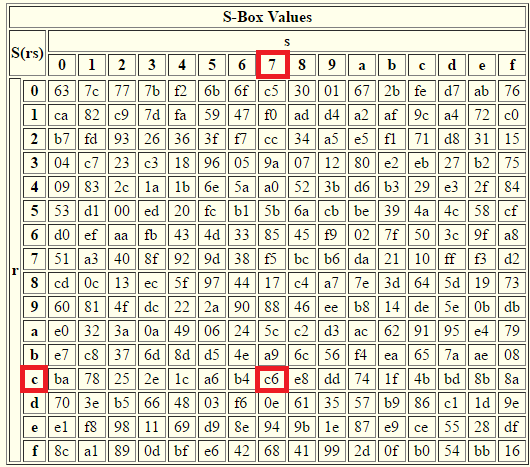
\includegraphics[scale=1]{SBox.PNG}
\caption{The lookup table used for AES, in hexadecimal notation\cite{SBox}.}
\end{figure}

A more memory efficient implementation can also be used instead of having to save a lookup table. There is also a formula, explained below, for calculating the byte with which a byte will be replaced when using an S-box. 

First, the multiplicative inverse of the byte is calculated within Rijndael's finite field (see 2.2.2.2). This multiplicative inverse, also a byte, is then stored as a vector $[x_7; x_6 ... x_0]$ to be used in an affine transformation.

\[ \left( \begin{array}{cccccccc}
1 & 0 & 0 & 0 & 1 & 1 & 1 & 1 \\
1 & 1 & 0 & 0 & 0 & 1 & 1 & 1 \\
1 & 1 & 1 & 0 & 0 & 0 & 1 & 1 \\
1 & 1 & 1 & 1 & 0 & 0 & 0 & 1 \\
1 & 1 & 1 & 1 & 1 & 0 & 0 & 0 \\
0 & 1 & 1 & 1 & 1 & 1 & 0 & 0 \\
0 & 0 & 1 & 1 & 1 & 1 & 1 & 0 \\
0 & 0 & 0 & 1 & 1 & 1 & 1 & 1\end{array} \right)
\cdot
\left( \begin{array}{c}
x_0 \\
x_1 \\
x_2 \\
x_3 \\
x_4 \\
x_5 \\
x_6 \\
x_7\end{array} \right)
\bigoplus
\left( \begin{array}{c}
1 \\
1 \\
0 \\
0 \\
0 \\
1 \\
1 \\
0\end{array} \right)
=
\left( \begin{array}{c}
b_0 \\
b_1 \\
b_2 \\
b_3 \\
b_4 \\
b_5 \\
b_6 \\
b_7\end{array} \right)
\]

So, after being manipulated by the S-Box, the byte of the state is replaced by the byte $[b_7; b_6 ... b_0 ]$. This step is performed for each of the 16 bytes in the state. After each byte of the state has been replaced, the new state continues on to the ShiftRows step.

\subsubsection{Transposition (SHIFTROWS)}
The next operation, transposition, operates upon the rows of the state by shifting each byte by a certain offset. The offset starts with 0, and is then increased by 1 for each row downwards from the top row.

\[ \left( \begin{array}{cccc}
a_{0,0} & a_{0,1} & a_{0,2} & a_{0,3} \\
a_{1,0} & a_{1,1} & a_{1,2} & a_{1,3} \\
a_{2,0} & a_{2,1} & a_{2,2} & a_{2,3} \\
a_{3,0} & a_{3,1} & a_{3,2} & a_{3,3}\end{array} \right)
\xrightarrow{\text{ShiftRows}}
\left( \begin{array}{cccc}
a_{0,0} & a_{0,1} & a_{0,2} & a_{0,3} \\
a_{1,1} & a_{1,2} & a_{1,3} & a_{1,0} \\
a_{2,2} & a_{2,3} & a_{2,0} & a_{2,1} \\
a_{3,3} & a_{3,0} & a_{3,1} & a_{3,2}\end{array} \right)
\]

\subsubsection{Substitution using formula (MIXCOLUMNS)}
The MixColumns step replaces each byte in the state with a different byte, dependent on all the bytes of that same column. All operations are performed within a finite field $GF(2^8)$.

In the MixColumns step, each column (and crucially not each individual byte) is treated as a polynomial Over $GF(2^8)$. This field is different from the Rijndael field, since it employs the reducing polynomial $x^4+1$ instead of $x^8+x^4+x^3+x+1$. This is because the column (which contains four values) will be represented as a third-order polynomial\cite{Rijndael}.
They are then multiplied, modulo the reducing polynomial, with a fixed polynomial $c(x)=03*x^3+01*x^2+01*x+02$. This process can also be shown by treating the column as a vector, and multiplying it with a special matrix:

The column (treated as a vector) is multiplied with a circulant (meaning that each row of the matrix is identical to the one above it, except that the values are offset by 1 to the right) MDS ("maximum distance separable", a representation of a function known to have useful properties in cryptography) Matrix \cite{MixColumns}.

It is very important to note that the values of the cyclical MDS matrix are not regular numbers, but actually represent hexadecimal bytes (for example, $03 = 11$, which is then padded with zeroes until it possesses 8 values, making it 00000011. This is permissible in Rijndael's finite field, as $11 = x+1 = 00000011$)

\[ \left( \begin{array}{cccc}
02 & 03 & 01 & 01 \\
01 & 02 & 03 & 01 \\
01 & 01 & 02 & 03 \\
03 & 01 & 01 & 02\end{array} \right)
*
\left( \begin{array}{c}
a_0 \\
a_1 \\
a_2 \\
a_3\end{array} \right)
=
\left( \begin{array}{c}
s_0 \\
s_1 \\
s_2 \\
s_3\end{array} \right)
\]

Now, it becomes evident that each byte of the resulting column is dependent on every byte of the manipulated column. As always, all operations take place in Rijndael's finite field. \\
\\
$
s_0 = {02}*a_0+{03}*a_1+{01}*a_2+{01}*a_3 \\
s_1 = {01}*a_0+{02}*a_1+{03}*a_2+{01}*a_3 \\
s_2 = {01}*a_0+{01*}a_1+{02}*a_2+{03}*a_3 \\
s_3 = {03}*a_0+{01}*a_1+{01}*a_2+{02}*a_3 \\ $

It is important to note that the last round of AES does not possess a MixColumns step; this is because, if there were a MixColumns step included in the last round of encryption, it would not possess a corresponding invMixColumns in the final round of decryption\cite{NoMixColumns}.

\subsubsection{Round-closing XOR operation (ADDROUNDKEY)}
Finally, the state is added to the round's unique round key using modular addition. The method is the same as described in chapter 2.2.2; an XOR gate is, once again, utilized.

\section{Decryption}
Just like encryption, decryption also begins with key expansion. Because the algorithm used is exactly the same as in encryption, the same round keys will once again be generated using the same master key that was already used for encryption. While each decryption round contains the inverses of the steps used in encryption, it is important to note that the order in which these steps appear in the rounds is not identical to the order in which their non-inversed counterparts appear in encryption.

\subsection{Initial inverse XOR operation}
Since all steps in decryption are the exact inverse of the encryption steps, the last round key used in encryption is used first in decryption\cite{RoundKeyInverse}. The inverse of the XOR operation is, fortunately, also simply the XOR operation. The following example demonstrates how adding the same key twice yields the same state as before having added the key.

\[
\left( \begin{array}{cccc}
1 & 0 & 1 & 1 \\
+ & + & + & + \\
0 & 1 & 1 & 0 \\
= & = & = & = \\
1 & 1 & 0 & 1 \\
\end{array} \right)
\]

\[
\left( \begin{array}{cccc}
1 & 1 & 0 & 1 \\
+ & + & + & + \\
0 & 1 & 1 & 0 \\
= & = & = & = \\
1 & 0 & 1 & 1 \\
\end{array} \right)
\]

\subsection{Rounds}
Just like in encryption, decryption consists of on initial inverse add round key step, followed by ten rounds, with the last round missing the inverse MixColumns step.

\subsubsection{INVERSE SHIFTROWS}
The Inv. ShiftRows step is rather simple, as it simply performs the exact opposite manipulation of the regular ShiftRows step.

\[
\left( \begin{array}{cccc}
a_{0,0} & a_{0,1} & a_{0,2} & a_{0,3} \\
a_{1,1} & a_{1,2} & a_{1,3} & a_{1,0} \\
a_{2,2} & a_{2,3} & a_{2,0} & a_{2,1} \\
a_{3,3} & a_{3,0} & a_{3,1} & a_{3,2}\end{array} \right)
\xrightarrow{Inv. ShiftRows}
\left( \begin{array}{cccc}
a_{0,0} & a_{0,1} & a_{0,2} & a_{0,3} \\
a_{1,0} & a_{1,1} & a_{1,2} & a_{1,3} \\
a_{2,0} & a_{2,1} & a_{2,2} & a_{2,3} \\
a_{3,0} & a_{3,1} & a_{3,2} & a_{3,3}\end{array} \right)
\]

\subsubsection{INVERSE SUBBYTES}
Just as in the regular SubBytes step, a lookup table is usually utilized in any practical implementations. The lookup table is generated using the following Process:

First, the inverse of the affine transformation performed in encryption is calculated and stored in a byte $[x_7;x_6...x_0]$. For the byte $[b_7;b_6...b_0]$, the inverse affine transformation is performed as follows:

\[ 
\left( \begin{array}{c}
x_0 \\
x_1 \\
x_2 \\
x_3 \\
x_4 \\
x_5 \\
x_6 \\
x_7\end{array} \right)
=
\left( \begin{array}{cccccccc}
0 & 1 & 0 & 1 & 0 & 0 & 1 & 0 \\
0 & 0 & 1 & 0 & 1 & 0 & 0 & 1 \\
1 & 0 & 0 & 1 & 0 & 1 & 0 & 0 \\
0 & 1 & 0 & 0 & 1 & 0 & 1 & 0 \\
0 & 0 & 1 & 0 & 0 & 1 & 0 & 1 \\
1 & 0 & 0 & 1 & 0 & 0 & 1 & 0 \\
0 & 1 & 0 & 0 & 1 & 0 & 0 & 1 \\
1 & 0 & 1 & 0 & 0 & 1 & 0 & 0\end{array} \right)
*
\left( \begin{array}{c}
b_0 \\
b_1 \\
b_2 \\
b_3 \\
b_4 \\
b_5 \\
b_6 \\
b_7\end{array} \right)
+
\left( \begin{array}{c}
0 \\
0 \\
0 \\
0 \\
0 \\
1 \\
0 \\
1\end{array} \right)
\]

Finally, the multiplicative inverse of the byte $[x_7;x_6...x_0]$ is found in Rijndael's finite field. This process is applied until all 16 bytes of the state have been replaced.

\subsubsection{INVERSE ADDROUNDKEY}
Since the inverse of an XOR addition is also the XOR addition (see 2.3.1), this step simply consists of adding the inverse round key to the state. For example, round key 9 would be the first round key to be added to the state, since round key 10 will already have been used in the initial inverse XOR operation\cite{RoundKeyInverse}.

\subsubsection{INVERSE MIXCOLUMNS}
The final step of each decryption round, except the last decryption round, is the Inv. MixColumns operation. The Inv. MicColumns step is performed by multiplying every column of the state with a specific polynomial d(x)\cite{Rijndael}. Once again, it is important to note that each column is seen as a third-order polynomial in $GF(2^8)$, with the reducing polynomial $x^4+1$ (see 2.2.2.6).

$d(x)$ has to be the inverse of the fixed polynomial used in the regular MixColumns step, $c(x)$, so it can be calculated in the following way:

\noindent
$c(x)*d(x)=01 \\
(03*x^3+01*x^2+01*x+02)*d(x)=01 \\
\Rightarrow d(x)=0B*x^3+0D*x^2+09*x+0E$

Just like the regular MixColumns operation, the Inv. MiColumns operation can also be performed by viewing the column to be replaced as a vector, and then multiplying it with a special matrix. This matrix is also the inverse of the matrix used in the regular MixColumns step.

\[ \left( \begin{array}{cccc}
0E & 0B & 0D & 09 \\
09 & 0E & 0B & 0D \\
0D & 09 & 0E & 0B \\
0B & 0D & 09 & 0E\end{array} \right)
*
\left( \begin{array}{cccc}
02 & 03 & 01 & 01 \\
01 & 02 & 03 & 01 \\
01 & 01 & 02 & 03 \\
03 & 01 & 01 & 02\end{array} \right)
=
\left( \begin{array}{cccc}
01 & 00 & 00 & 00 \\
00 & 01 & 00 & 00 \\
00 & 00 & 01 & 00 \\
00 & 00 & 00 & 01\end{array} \right)
\]

\[ \left( \begin{array}{cccc}
0E & 0B & 0D & 09 \\
09 & 0E & 0B & 0D \\
0D & 09 & 0E & 0B \\
0B & 0D & 09 & 0E\end{array} \right)
*
\left( \begin{array}{c}
s_0 \\
s_1 \\
s_2 \\
s_3\end{array} \right)
=
\left( \begin{array}{c}
a_0 \\
a_1 \\
a_2 \\
a_3\end{array} \right)
\]

\section{Fulfilment of Shannon's properties}
In 1945, Claude Shannon wrote a report that would become central to cryptography. This report was titled "A Mathematical Theory of Cryptography", and it identified two properties necessary to ensure the security of any cipher\cite{ShannonProperties}. These were termed diffusion and confusion. These two properties, if fulfilled, serve to make methods of cryptanalysis, in particular statistical analysis, less effective.

\subsection{Diffusion}
Diffusion requires that, as a rule of thumb, changing one bit of the plaintext should alter half of the ciphertext, with the reverse also being true; this is referred to as the avalanche effect\cite{AvalancheEffect}. This is best achieved by spreading the values of the plaintext out over the entire ciphertext; hence the term "diffusion".

In AES, diffusion is  provided by the MixColumns and the Shiftrows steps. The diffusion provided by the ShiftRows step is self-evident; as the bytes are entered into the state in a column-major order, mixing the bytes along the rows is a good source of diffusion.

MixColumns is a good source of diffuion because it creates a dependecy of four bytes on just one byte; if a single byte of the four substituted bytes are changed, every byte resulting from the substitution is also changed. This effect is further compounded because it is performed nine times, meaning that if just one bit, contained within a byte, of the initial plaintext is altered, the ciphertext will be dramatically different.

\subsection{Confusion}
Confusion requires that each bit of the ciphertext relies on multiple different parts of the key. This means that the input data must be altered in a non-linear, difficult to reverse manner, thereby obscuring the relation between the ciphertext and the key\cite{Confusion}.

In AES, confusion is provided by the SubBytes step. This can be seen if the journey of a single byte through AES is examined; Since each byte goes through so many substitutions, it is difficult to find the key even if one were to possess a large number of plaintext-ciphertext pairs.

\section{Problems with AES}
In 1997, NIST deemed it necessary to replace DES, the data encryption standard, with AES, the advanced encryption standard, because of DES' vulnerability to brute force attacks due to its small key size. 15 submissions were received, but Rijndael was selected due to its good performance and security\cite{AESSelection}.

Though AES was thouroughly vetted during the AES selection process and is considered secure enough to be used in encryption of top secret documents by the National Security Agency\cite{CNSSPolicy} of the united states, it is unfortunately not perfect.

\subsection{Overconfidence and over-reliance}
AES is widely used by large businesses and the United States government. Therefore, it would be a large threat to many nations national security if the Cipher were to be compromised.

One of the earliest scares was the XSL attack, which relied on the relative algebraic simplicity of AES\cite{XSL}.However, this proposed attack was later shown to be technically infeasible\cite{XLSRebuked}; nevertheless, this shows that while AES is very secure, the cryptographic community must remain vigilant in its continued research into possible attacks in order to ensure the security of highly sensitive data across the world.

\subsection{Keeping of a shared secret}
One of AES' major issues is shared with OTP and all other symmetric-key encryption methods; the confidentiality of the key. The same argument that was made against OTP can be made against AES as well, namely that because the encryption method as well as the decryption method are both publicly known, the problem of keeping the message or file secret is simply transferred to keeping the key secret, while still being able to exchange it between the sender and the recipient.

However, in the case of AES, this issue is strongly mitigated: While the key used in OTP has to be at least as long as the message, AES keys are only 128, 192 or 256 bits long, with top secret documentation requiring the usage of either a 192 or 256-bit key\cite{CNSSPolicy}.

\chapter{A historical transition}
Throughout modern history, cryptography has always been an essential part of our lives. From warfare to communication and economy, many of recent histories most momentous occurrences have been influenced by cryptography. This is especially true in the case of OTP and AES; one having played a key role in WWII, the largest military conflict of human history, the other being implemented as a standard just shortly before cryptography was brought to the public eye like never before through numerous security breaches, conspiratorial government spy programs and the new dangers of a globalist economical system. In order to learn from history and apply it to present issues, it is essential to examine the first computer-aided cryptography system using the mechanical Vernam machine and representing bits using punch cards\cite{VernamMachine}, OTP, and understand how it differs from but also inspired certain elements of today's standard, AES, which uses modern computers.

\section{Key differences and improvements}
While OTP was a building block of the foundation of modern computational cryptography, AES and the algorithms which support it in regular use currently stand at its pinnacle. With many different implementations and possible uses, each one of them tailored to achieve a specific goal and ongoing research and development, AES is truly on the cutting edge of cryptography. Many of its great achievements are great improvements over earlier algorithms, as well as a degree of flexibility that has seldom been observed within cryptographic algorithms.

\subsection{Memory vs. computational efficiency}
One of the greatest advantages of AES, which is not at all present in the case of OTP, is its ability to be implemented in a way that is either computationally or memory efficient. 

Almost all operations performed in AES can be pre-saved, for example in the case of lookup tables (see 2.2.2.4). This also applies to the key expansions step (see 2.2.2.3), as all Rcon vectors can either be pre-calculated and stored or calculated during runtime of the algorithm. This even applies to the MixColumns step (see 2.2.2.6); although the lookup table would be very large, pre-calculating and subsequently storing it would make the algorithm run very quickly.

On the other hand, it is also possible to make each calculation completely without lookup tables, storing only the currently needed value, be it a number, vector or matrix, at one time. This is computationally rather taxing, however extremely memory-efficient as the algorithm only requires its source code and a very small storage block to function.

This flexibility in implementation is one of AES' greatest advantages, especially when compared with the rigid requirements of OTP.

\subsection{Key length}
The most relevant improvement AES makes over OTP, as well as many other contemporary ciphers such as RSA which requires a minimum key length of 1024 bits, is its short key. AES manages to retain the great security benefits that can be achieved by using a secret key, whilst also substantially shortening the key. The master key, although short, retains great cryptographical power because of AES' usage of KeyExpansions(see 2.2.2.3). This is a large advantage in today's time-critical society and economy: a short key is faster to generate and easier to transport or transmit. Furthermore, an AES key can be reused multiple times, unlike OTP, where the key must be discarded after one use.

%Furthermore, This enables the key to be sent over the internet more easily, using other encryption methods to protect the key itself. This is in contrast to keys for OTP, which are usually transported physically by courier.

\section{Key similarities and inspirations}
Many of AES' most important elements take heavy inspiration from OTP. This comes as no great surprise, considering that though cryptography has long been evolving, it has always strived to achieve the same goals. The following chapter will serve to highlight the similar methods used in OTP and AES to achieve those goals.

\subsection{Key addition}
The only encrypting measure performed in OTP is an XOR addition of the key and the plaintext. While AES performs many different cryptographical measures, one of its absolute core principles is still the employment of a secret key, making it a symmetrical secret key algorithm, just like OTP. In this way, AES has taken inspiration from OTP whilst also improving one of OTP's major weaknesses: Its key length.

After all, one of OTP's great weaknesses is that the key is equally as long as the message. Many critics have argued that this simply transfers the problem of transporting the secret message to the transport of the secret key. However, this can be combatted:

After all, the key is not actually secret until it has been conclusively employed. One method is to continue attempting to send keys until one manages to reach its destination without being compromised. At this point, the message can be encrypted using the uncompromised key and sent to the reciever.

\subsection{Secure transmission methods}
As aforementioned, one way to combat the issues caused by OTP's large key length is to continue sending keys until a key arrives uncompromised at the ciphertext's intended recipient.

\begin{center}
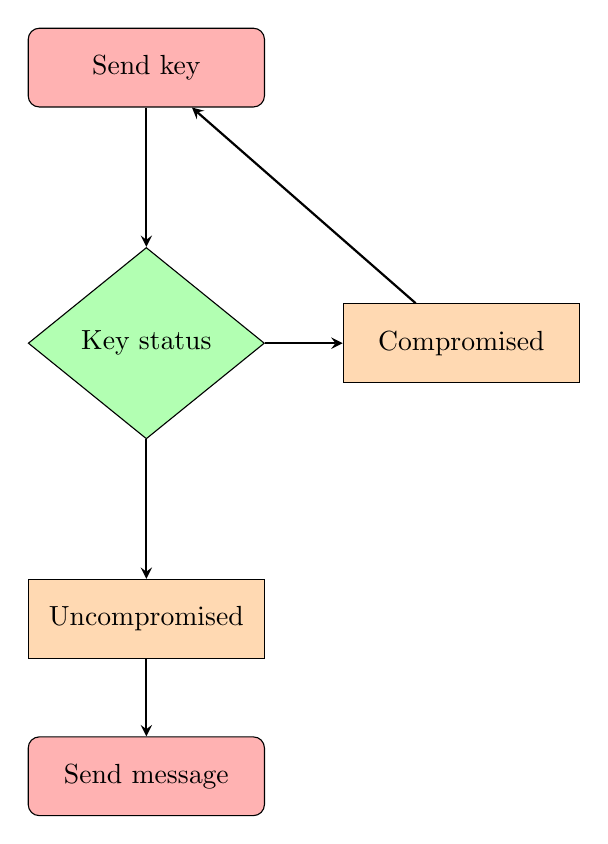
\begin{tikzpicture}[node distance=2cm]
\node (start) [startstop] {Send key};
\node (dec1) [decision, below of=start, yshift=-1.5cm] {Key status};
\node (proc1) [process, below of=dec1, yshift=-1.5cm] {Uncompromised};
\node (proc2) [process, right of=dec1, xshift=2cm] {Compromised};
\node (end) [startstop, below of = proc1] {Send message};
\draw [arrow] (start) -- (dec1);
\draw [arrow] (dec1) -- (proc1);
\draw [arrow] (dec1) -- (proc2);
\draw [arrow] (proc2) -- (start);
\draw [arrow] (proc1) -- (end);
\end{tikzpicture}
\end{center}

Interestingly, this has made it possible for OTP to make a comeback in the modern high-security industry: With the advent of hard drives able to store vast amounts of information, keys as large as 3TB can be transported in relative secrecy. This, coupled with new high-speed random number generation techniques such as atmospheric noise\cite{RandomOrg}, enable the creation and covert transportation of extremely long random keys. If one such hard drive is successfully transported to a recipient, with a sender retaining an identical copy, they will be able to send 3TB of text, amounting to a large amount of messages, securely between each other until the length of the key is exhausted.

Therefore, an advantage of OTP can be paraphrased as "the movement of perfect secrecy through time". If a secure channel can only be accessed for a limited amount of time, the sending of a large key can enable later secure communication, even over insecure channels.

In order to transmit a secret key, of course necessary in the case of AES, between two parties over an insecure channel such as the internet, the Diffie-Hellman key exhange algorithm is utilized. However, it is not completely accurate to say that the key is "transmitted"; rather, each party individually generates the same key \cite{DiffieHellman}.

First, two prime numbers are generated, for example $a$ and $m$. These are shared between the two parties.

Next, the first party generates a secret number $c$, which will remain known only to the first party. They then compute $a^c mod m = C$. $C$ is sent to the second party.

The second party now generates a secret number $d$, which will remain known only to the first party. They then compute $a^d mod m = D$. $D$ is sent to the first party.

The first party, having received $D$, now performs the same operation again, using their secret number:
$D^c mod m$

The second party, having received $C$, now performs the same operation again, using their secret number:
$C^d mod m$

The brilliance in this algorithm lies in the fact that each party will receive the same number from their respective final operations; this is due to a special property of exponents in conjunction with modular operation, namely:

$(a^c mod m)^d mod m = a^{cd} mod m$
$(a^d mod m)^c mod m = a^{dc} mod m$

This method is secure because the two generated secret numbers, $c$ and $d$, were never transmitted between the two parties.

\section{Cryptography: Past, present and future}

\subsection{The modern war}
With the recent revelations brought about through the Snowden scandal\cite{Snowden}, cryptography as a tool of the state has become a theme of major public interest in a way that has not seen precedent since the second world war.

This is one of the major reasons OTP and AES are definitely comparable in a historical context; they were both relevant on a global scale, being used in covert high-security operations, deciding the fates of countless individuals, even perhaps lending a decisive advantage to those most proficient in their employment.

The British intelligence community in particular played a huge role in the allied victory. Much of this sucess is attributed to Alan Turing, who provided extremely significant advances in the battle to crack the German enigma system\cite{AlanTuring}. However, another fact that must not be glossed over is the sucessful employment of OTP by the British Special Operations Executive, which enabled slow yet extremely secure communications, even being employed amongst field agents towards the later years of the war.

AES now finds itself a key element in a different kind of, yet equally important for mankinds future, conflict. With the advent of globalism, the battle for economic, ideological and social supremacy has grown fiercer and more multi-faceted than ever. This, coupled with the United States position as the globes sole superpower waning, in fact being contested by China and Russia's rise out of communism into extreme capitalist competitiveness, makes information and intelligence more valuable than ever. Today's conflict is not concerned with large-scale troop movements and industrial weapons production, but instead with the passwords of CEO's, small-scale targeted tactical strikes and the economic plans of gigantic corporations.

This is where the relevance of AES becomes apparent. AES is widely utilized by the U.S and other governemts to encrypt files ranging from SECRET to TOP SECRET security clearance\cite{CNSSPolicy}. However, unlike OTP during the second world war, AES also plays a large role in the lives of regular people, as techonology has become ever more integrated into our daily lives: For example, many websites using https (hyper-text transfer protocol secure) use 128-bit AES encryption in conjunction with Diffie-Hellman key exchange. Any entity able to somehow crack or bypass AES would have access to an unimaginably large quantity of valuable information. The many large corporations which employ modern cryptography include PayPal, a company which processed more than 87 billion dollars in the third quarter of 2016 \cite{PayPal}, use 128-bit AES encryption.

\begin{figure}[H]
\centering

\includegraphics[scale=0.3]{PayPal.png}
\caption{Google Chrome can show which encryption standard a certain website is utilizing.}
\end{figure}

Given these new developments, it is certainly fair to say that cryptography plays a more important role in the lives of everyday people than ever before in human history.

\subsection{Privacy: An outdated concept?}
With new and exciting developments that have inseparably linked technology and social media to the lives of billions of ordinary people across the globe, many exciting new possibilities have been realized. Seamlessly integrating into our daily routine, services such as google calendar enable us to plan our day, while all transactions can be taken care of over services such as PayPal or Samsung Pay with nothing but the press of a button. We can access the knowledge of the entire world or connect with others across the globe using a device that fits in our pocket.

However, in using these revolutionary new technologies, we have been exposed to new risks and vulnerabilities, many of which are only just becoming apparent through the unpleasant revelations that recent years have brought. This is why cryptography is currently so important, and also why its relevance will only continue to grow as the rapid pace of technological development continues.

This growing importance of cryptography is why it is imperative not just for academics, but also for regular people to understand what cryptography is and how it functions. With most of our communication and financial transactions being conducted over the internet, we can no longer assume that privacy is our default state: Instead, we must remain vigilant in safeguarding it. To this end, we all use cryptography, whether we know it or not.

\section{Closing remarks}
In conclusion, the importance of cryptography is greater than ever before. Therefore, it is my strong belief that every person living and working in the modern world can profit greatly from understanding modern as well as historical cryptography, due to their highly important roles in our private and professional lives. To this end, I hope that this paper has succeeded not only in shedding some light upon the highly intricate algorithms that permeate our everyday existence, but perhaps also in igniting some spark of fascination in what I consider a highly important, yet rather under-examined facet of our daily lives.

In closing, I would like to leave you with thanks for reading, but also a final thought: Although the algorithms we use today are incredibly potent and secure, they too, just like AES' predecessor DES, are sure to be replaced. Therefore, the most important conclusion that can be drawn from this paper is not just the current importance of cryptography for us all, but the importance of staying informed, and continuing to strive to understand how our information is safeguarded, as well as the algorithms that undertake and will long continue to undertake this momentous task.

% have to print the bibliography once all entries are made, otherwise an error keeps occuring.
\printbibliography

\end{document}

